\section{Track reconstruction}
\label{sec:track_reconstruction}

	The time between the track hit time stamp and the signal rising edge is a measure of {\it drift time} of these electrons. The relation between the   {\it drift time} and  the distance from the track to the center of the tube(wire while no sag for centered wire) is called {\it drift time - distance} relation or {\it tr-relation}.
	
	The drift time $t$ is a function of track position (relative to the wire) and electric field along the drift trajectory.
	
	One assumes that the working  position  for straws will be perpendicular to the particle flow, and  acceptance of particle spreading will not be significantly big. So tracks will be collinear each other within every separate  STRAW tube unit.
	
	Summing the above mentioned we have one dimension task -- reconstruct tracks on vertical axis\footnote{An example of single track reconstruction which explains the approximate procedure of reconstruction you can see on Fig.\ref{fig:track_reconstruction}}	(see examples of outcome tr-distribution $t = t(r,s=0)$ in Fig.\ref{fig:t_r_distr_00} and Fig.\ref{fig:tr_distr_15})  even the wire sagging. Sagging will be always down thanks to gravitation force $\vec{g}$.
	
	\begin{figure}[h!]
		\centering
		\subfloat[wire at the center]{
			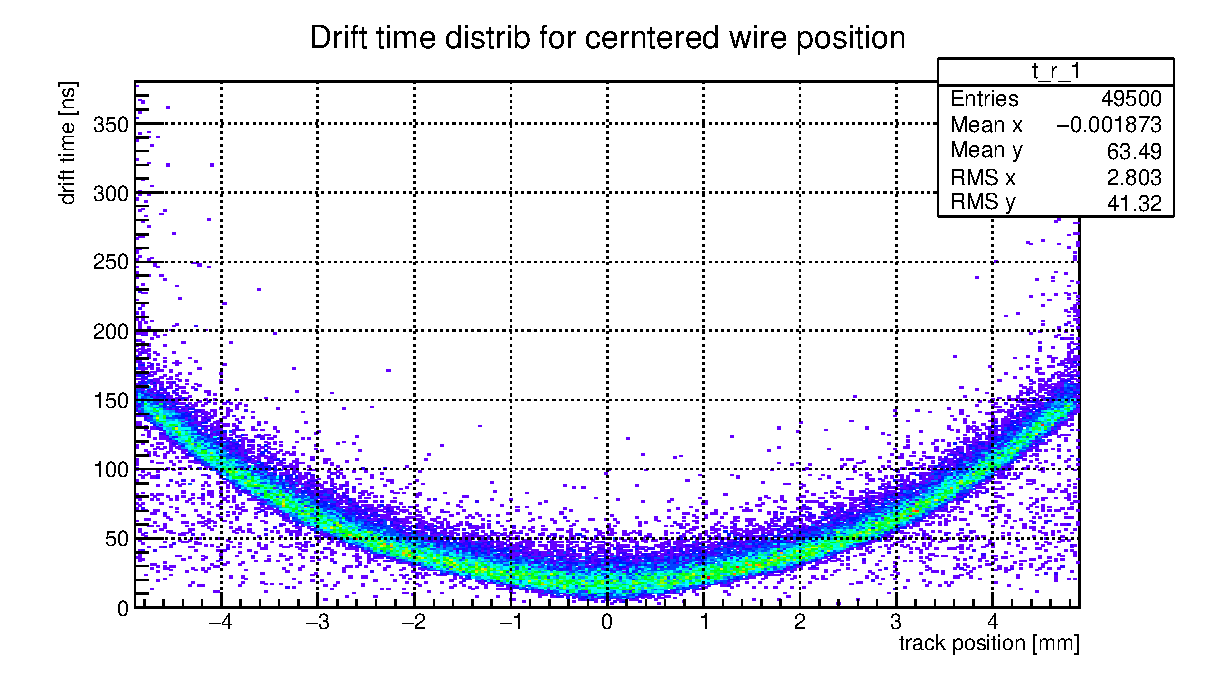
\includegraphics[width=0.45\textwidth]{t_r_distr_00} 
			\label{fig:t_r_distr_00} }%
		\qquad
		\subfloat[$1.5mm$  offset]{
			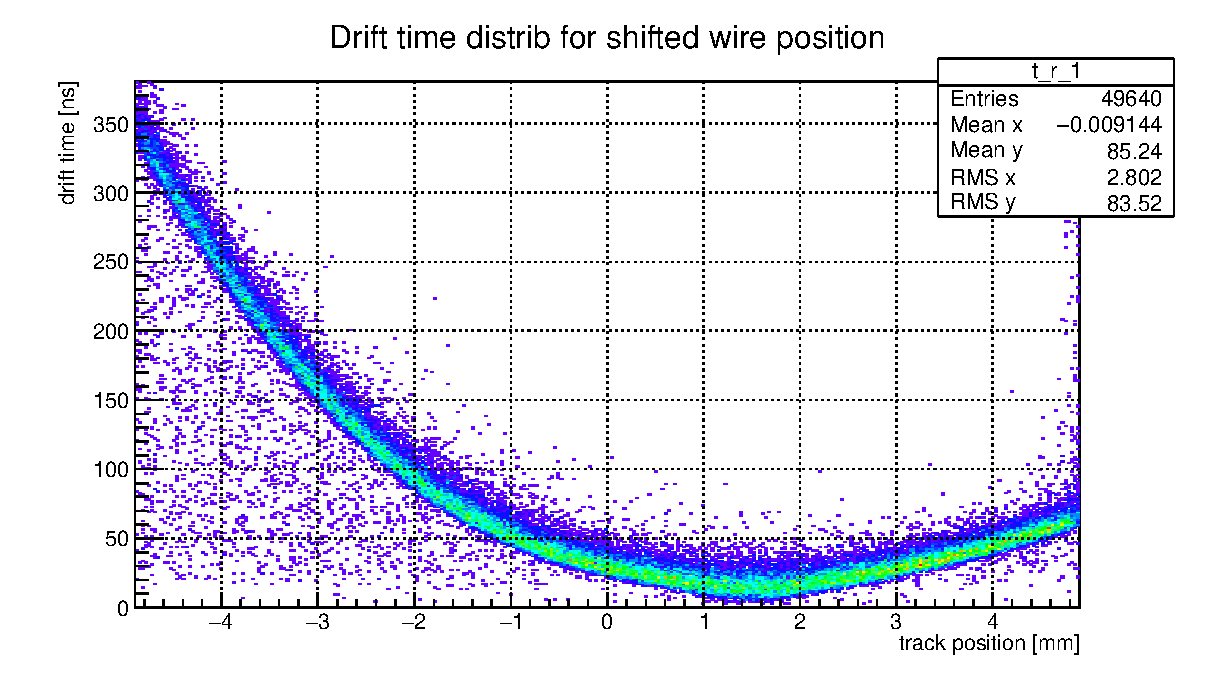
\includegraphics[width=0.45\textwidth]{tr_distr_15} 
			\label{fig:tr_distr_15} }%
		\caption{Distribution of drift time $t_{drift}$ as function of track position $r_{track}$ relatively to the tube center}			
	\end{figure}	
	
	The rt-relation varies along the tube according to wire displacement $s$. Thus we have for the drift time:
	\begin{equation}
	t_{drift} = t_{drift}(r_{track},s)
	\end{equation}
	
	The idea is to find the inverse dependence
	\begin{equation}
		r_{track} = r_{track}(t_{drift},s)
	\end{equation}
	
	From Sec.\ref{sec:sagEstimation} we can find sag profile for straw. Therefore the rt-calibration becomes 1 dimension less for every certain value of wire displacement $s_0$:
	\begin{equation}
		r = r(t,s=s_0)
	\end{equation}
	
	
	\subsection{How drift time resolution depends on wire offset?}
	
	Deformation of electric field inside the tube invoked by wire displacement from the center position affects drift time. Here we are going to estimate magnitude of drift time change.
	
	As was noted above we make a binning  for our data along the $r_{track}$ (Fig.\ref{fig:t_r_distr_00},\ref{fig:tr_distr_15}). Resolution equals to RMS at every bin of digram (Fig.\ref{fig:driftTimeResolutionEvo}).
	
	\begin{figure}[h!]
		\centering
		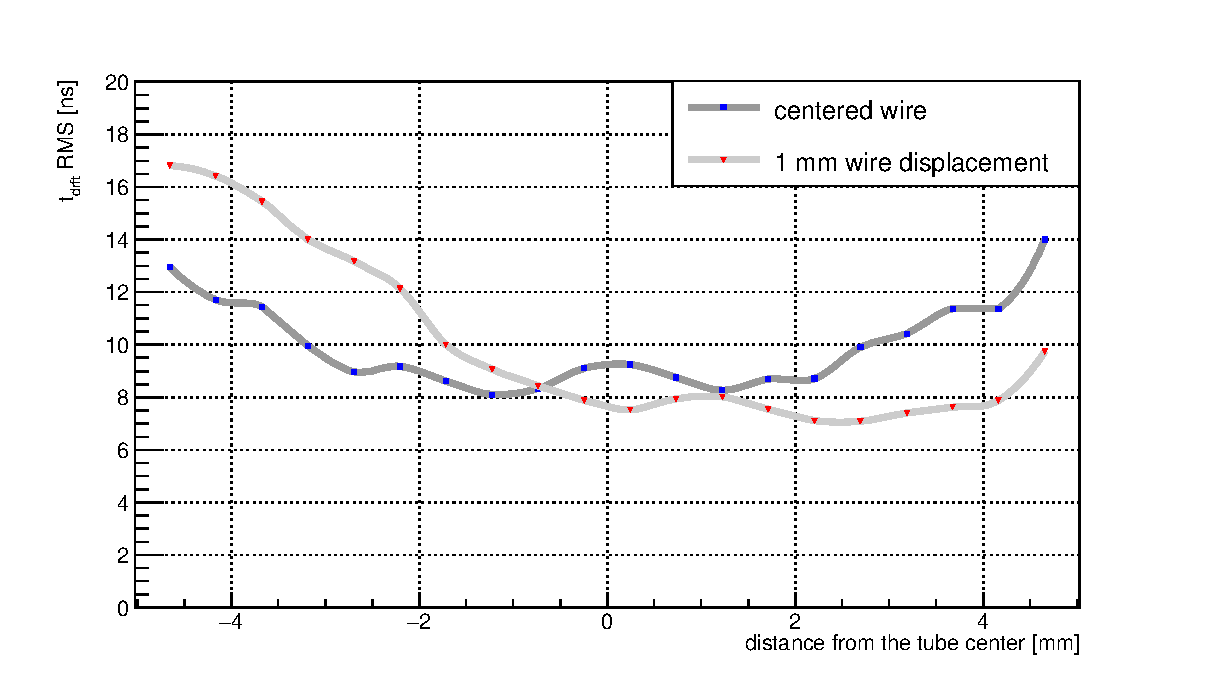
\includegraphics[width=0.9\textwidth]{DTimeRMS2}
		\caption{Resolution of drift time as a function of distance from the wire.}
		\label{fig:driftTimeResolutionEvo}
	\end{figure}
	
	We are dealing with probabilistic  nature of clustering that spread RT-relation from thin line. The leakage noise is also present in calculation but the effect is not very high (especially in this calculation).
	
	Every plot of output current (see fig. \ref{fig:signal_example}) consist of 1000 equidistant frames. The threshold is set to $5\sigma$ of noise. Leakage noise make effect on drift time measurements in case its amplitude becomes higher that threshold value in range from $t=0$ to $t= t_{drift}$. At five-sigma there is only one chance in nearly two million that a random fluctuation would yield the result. The drift time for tracks close to the tube edge can be up to $150 ns$ and $300 ns$ in case wire displaced. The probability to meet noise above threshold value is less than $0.02\%$.
	
	Another source of noise points on TR-distribution comes from $\delta$-electrons that cause secondary ionisation in tube volume. Only those electrons make impact which are emitted in the direction of the wire(see example on fig.\ref{fig:deltaElectron}).
	
	\begin{figure}[h!]
		\centering
		\subfloat[$\delta$-electron affects on drift time]{
			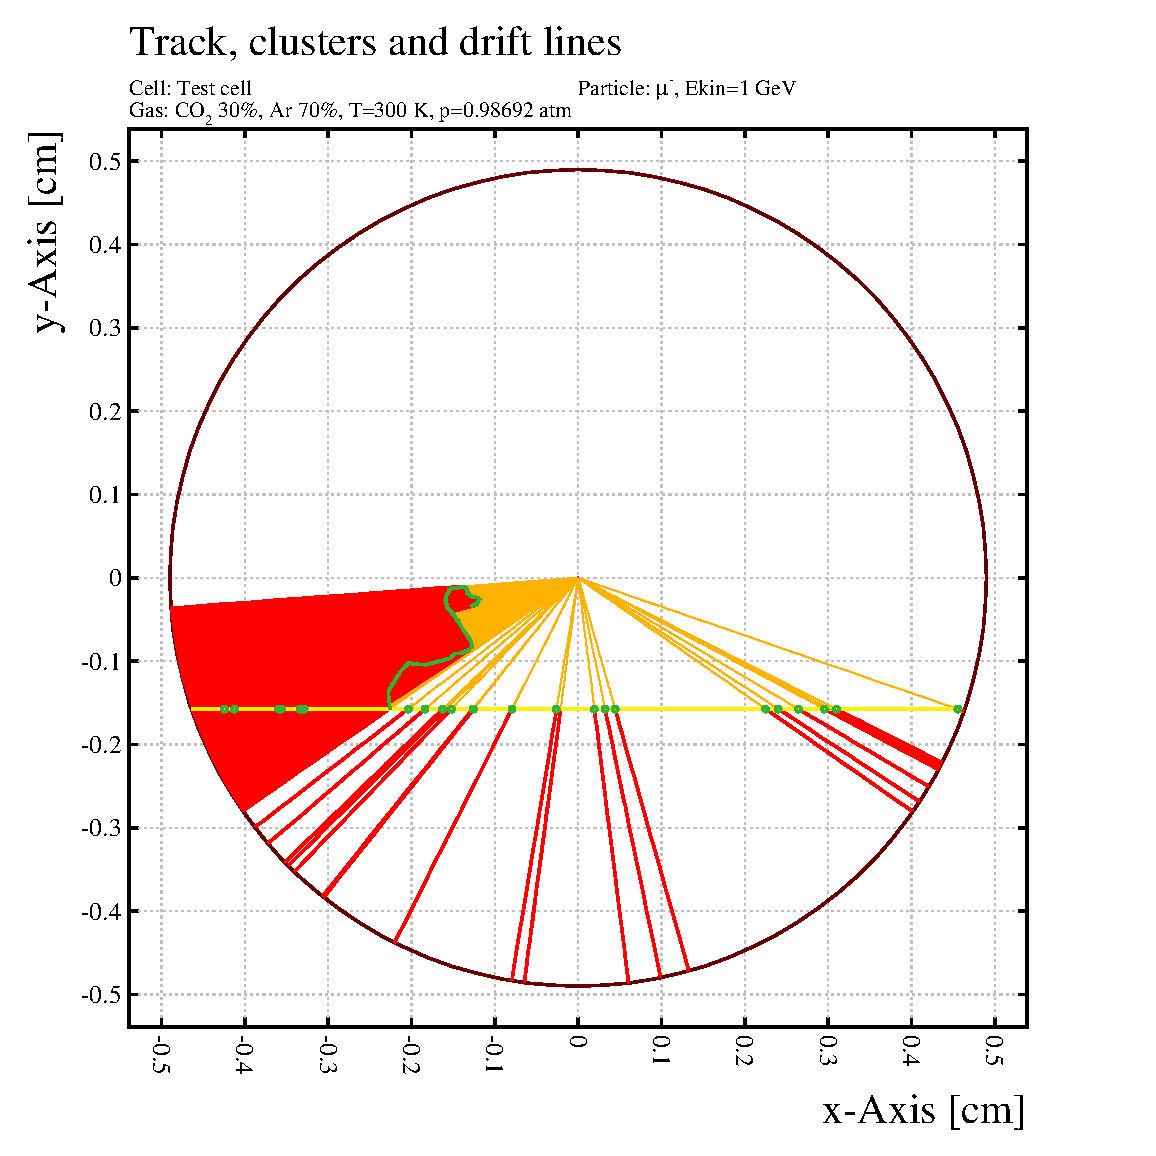
\includegraphics[width=0.45\textwidth]{deltaElectron} 
			\label{fig:deltaElectron} }%
		\qquad
		\subfloat[$\delta$-electron that moves away from the wire has no affect on drift time]{
			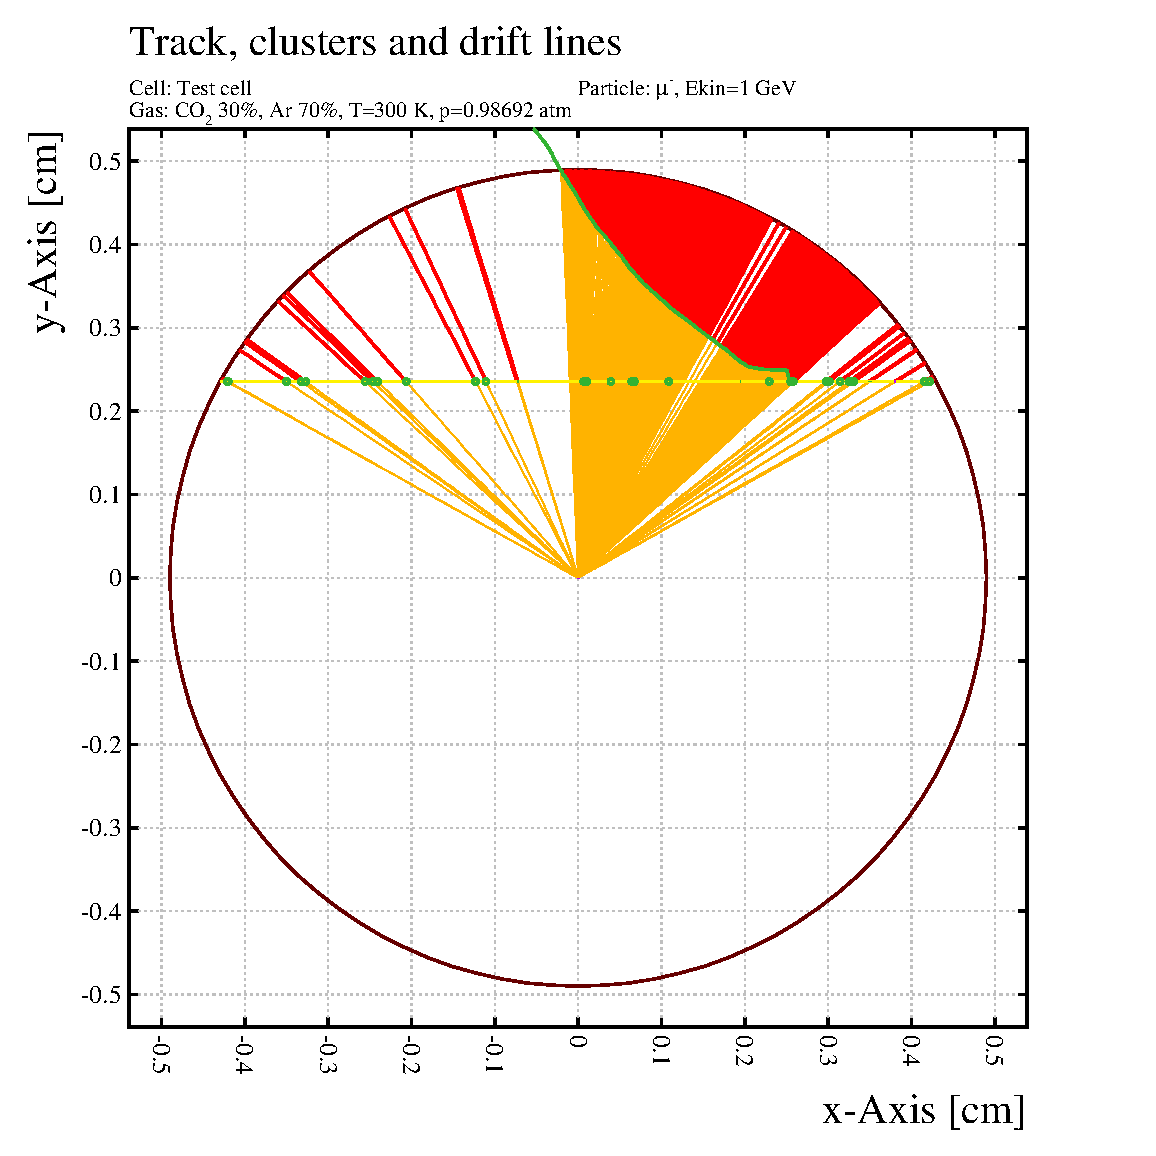
\includegraphics[width=0.45\textwidth]{deltaElectronNoEffect} 
			\label{fig:deltaElectronNoEffect} }%
		\caption{Garfield simulation with $\delta$-electron presence. Red lines - ion trajectory, yellow - electrons. Trajectory of $\delta$-electron marked by green curve line.}			
	\end{figure}	
	
	The number of events out of TR-ralation caused by $\delta$-electrons is quite small. Especially percentage of events where $\delta$-electrons make effect on drift time is less that $1\%$ of total number of events  in GARFIELD simulations. 
	
	Tube wall is very thin but particle still can cause $\delta$-electrons when crossing it. GEANT4 studies show that such kind effect also presents in interaction of muon with tube volume, and percentage of events with $\delta$-electron that affect drift time even less that $0.2\%$.
	
	\subsection{Finding of rt-relation}
	
	The RT-relation depicts relation between drift time and track position. The idea is to find the best fit of give data to achieve higher resolution and avoid systematic errors.
	
	The problem is in that we have to minimize influence of noise while fit. One suppose that the noise has approximately homogeneous distribution of points that locates below the main line of distribution. Consequently we can filter it by fitting only points from regions with local point density higher that some threshold value. Another way is to make a binning of our distribution along the track position and fit every 1D histogram by Gaussian. The fit points of Gaussian mean values by fit function.    
	
	Nevertheless our data contain very small amount of "non-track" points.
	
	TR-relation is asymmetry relatively to the $r=0$ almost in all cases except wire in the center of the tube. Therefore we have to calibrate for every of branches. It means we need to find two track positions for every of drift time value and reject one of them in further data processing stages.
	
	In previous section we found way to measure wire sag profile. So we can use this trick in present stage for separating data into ``right'' and ``left'' branch. Every of branches we will calibrate separately.
	
	Lets suppose we can fit every of TR-diagram by pair of analytic fit functions (\ref{eq:trRelation}):
	\begin{equation}
	t(r_{track}) = e^{a_0 + a_1r_{track}}
	\label{eq:trRelation}
	\end{equation}
	
	\begin{figure}[h!]
	\centering
	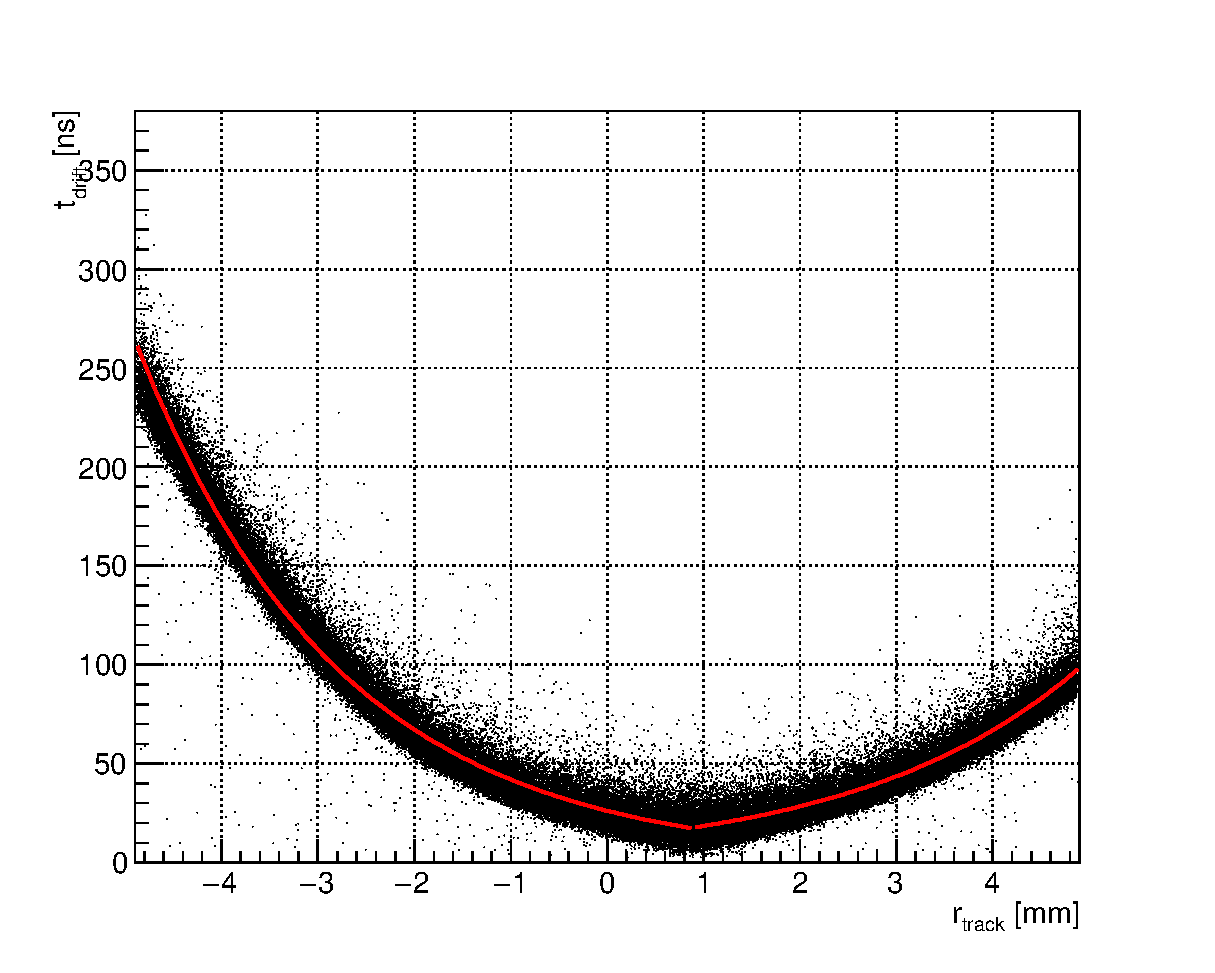
\includegraphics[width=0.7\textwidth]{TRrelation_09_points}

	\caption{TR-relation fitting for $0.9 mm$ wire offset value}
	\label{fig:TRrelation09p}
	\end{figure}
	
	If the Fig.\ref{fig:TRrelation09p} you can see TR-relation. Fitting is not perfect because of using simple fit function template (\ref{eq:trRelation}). But we will use reverse to the (\ref{eq:trRelation}) relation, because we have to find $r_{track}$ from known $t_{drift}$. We can do it be because the aim of this studies is not a precise calibration but global evaluation effect of wire sagging into total result.
	
	As you can see in the Fig.\ref{fig:TRrelation09p} red fit line does not cover whole drift time spectre. So events with drift time less than covered range(less than $\sim20 ns$) counts as track through the wire:
	\begin{equation}
	r_{track}(t_{drift} < t_{min}) = r_{wire~pos}
	\end{equation}
	where $t_{min} = min (t_{drift}(r_{track}))$, $r_{track} = \overline{(-r_{tube},r_{tube})}$. Respectively tracks with drift time higher than maximum of fit function range is artificially counted as tracks with near tangents to the tube position $r_{track} = \pm r_{tube}$  (because efficiency decreases near the tube wall down to $20\%$).
	
	\subsection{Track reconstruction precision}
	
	Obviously the precision is the main factor in design of detector.
	
	The STRAW tube tracker should be as light as possible to avoid multiple scattering on structural components of detector. But design should be changed within reason if precision suffers from this\footnote{Especially design with no sagging works well for experiment NA62 \cite{}. But they have more than 2 times shorter  straw when tube have insert in the middle of the tube. So sagging becomes negligible in this case.}.
	
	How precision of track reconstruction depends on wire position(wire displacement)?
	
	\begin{figure}[h!]
		\centering
		\subfloat[reconstructed track position $r_{rec}$ as function of true track position $r_{track}$]{
			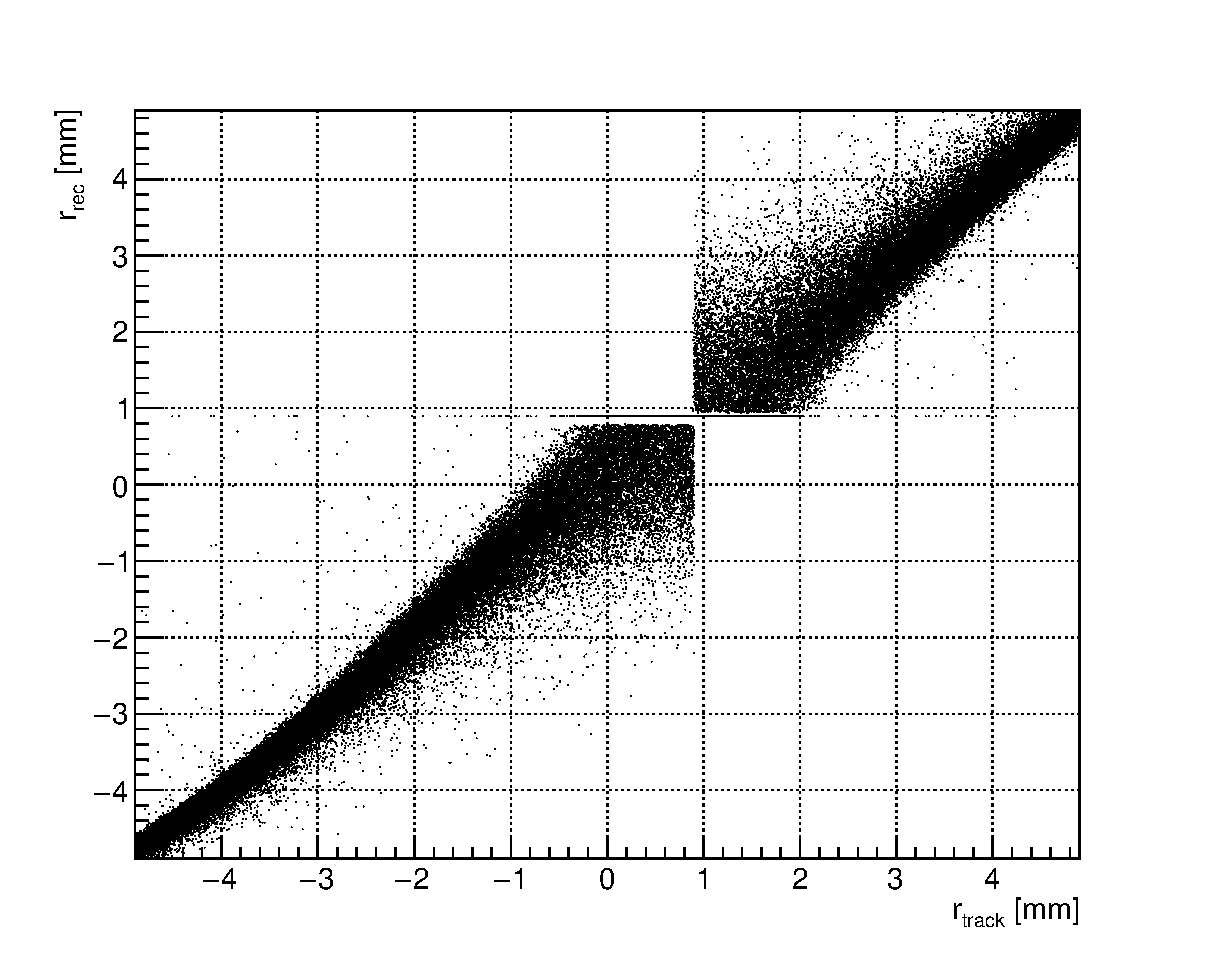
\includegraphics[width=0.4\textwidth]{reconstructed_points} 
			\label{fig:reconstructed_points} }%
		\qquad
		\subfloat[$r_{track} - r_{reconstructed}$ as function of $r_{track}$]{
			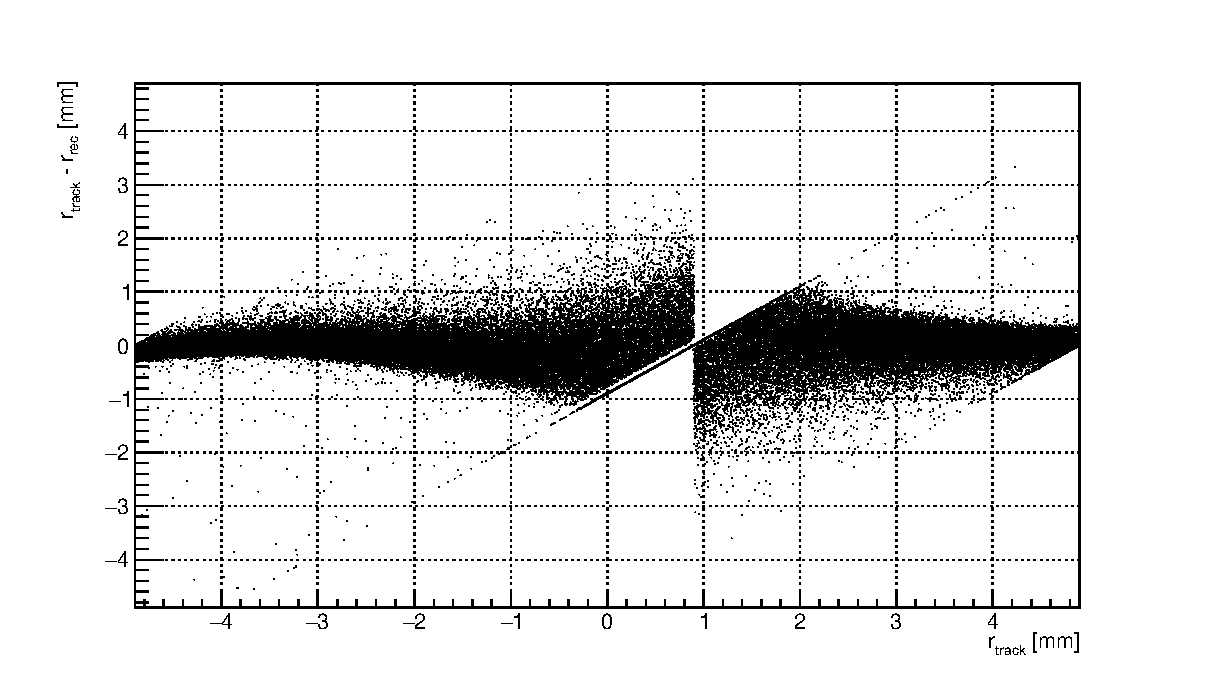
\includegraphics[width=0.5\textwidth]{diffRecTrue09_points} 
			\label{fig:diffRecTrue09_points} }%
		\caption{Distributions of matching of track position to their reconstructed value.}
	\end{figure}
	
	\begin{figure}[h!]
	\centering
	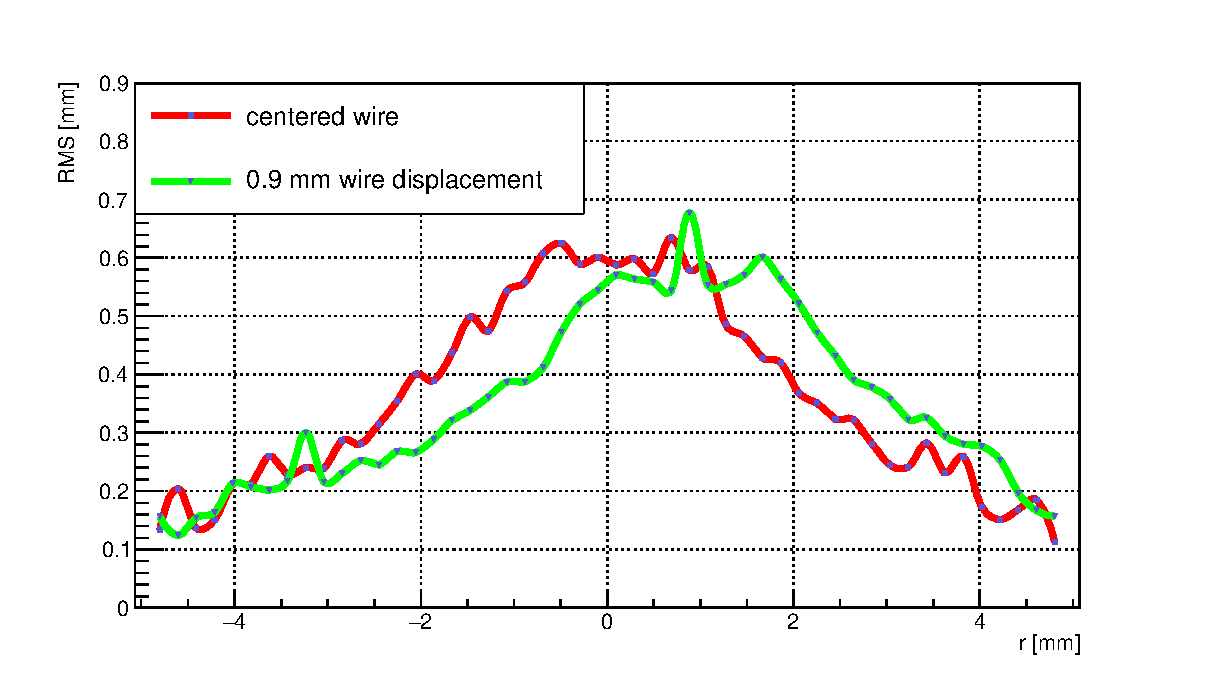
\includegraphics[width=0.9\textwidth]{precisionCompare_0_9}
	\caption{Comparison of track reconstruction precision for two wire position. Value of precision at every point means RMS of data sample near corresponding track position $r$. Red line corresponds to the centered wire position, green line -- to the $0.9 mm$ sagged wire  position.}
		
	\label{fig:precisionCompare09}
	
	\end{figure}
	
	As you can see on Fig.\ref{fig:precisionCompare09} there are no significant difference of track reconstruction precision between two mode of wire location despite of the increasing drift time for displaced wire position(with almost factor of two).	 The highest resolution($\sim 0.1 mm$) near the tube wall and worst value $\sim0.6mm$ is near the wire because the clustering effect. Higher gas pressure should resolve this problem.